\section{Introduction}

\begin{figure}[!tbh]  %[htbp]
%\vspace*{-0.1in}
  \begin{center}
       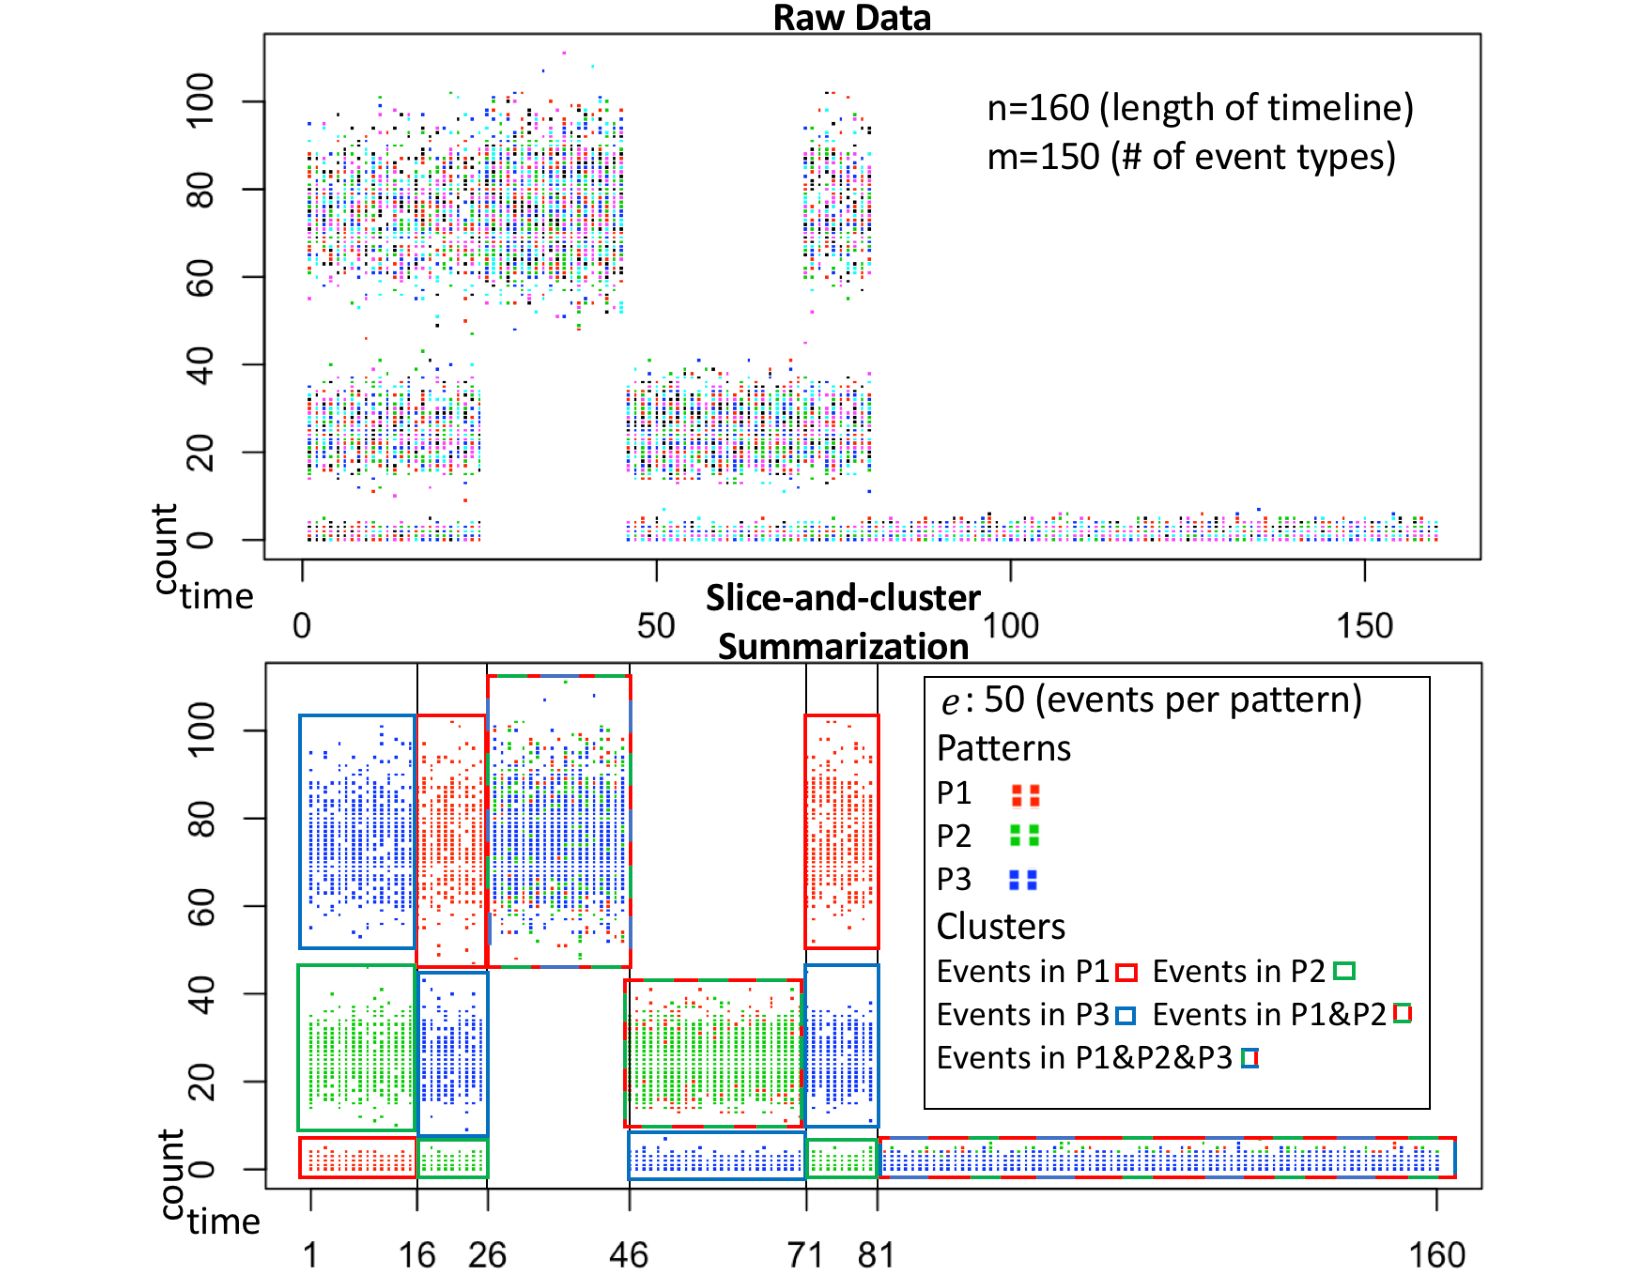
\includegraphics[trim = 0.5in 0in 0in 0in, clip,scale=0.35]{images/intro.pdf}
  \end{center}
%  \vspace{-0.2in}
   \caption{The raw data in the top figure shows a timeline by day, from 1 to 160. Each dot in the raw data, represents a daily event frequency from 150 events. These events follow group patterns identified by the Slice-and-cluster summarization in the bottom figure. The output of the summarization is, first, the segmentation of the time dimension \{1-15, 16-25, 26-45, 46-70, 71-80, 81-160\} and second, the local clusters for each of these time segments. Each local cluster is a list of events id's that form part of the cluster and the summarization is a daily rate. Because this is synthetic data we know the list of events that conforms a pattern, and the algorithm accurately detects them. For visual aid the local clusters are represented by a color box of the pattern an event belongs to, if the events are all from different patterns but can be represented by the same daily rate the color boxes are combined.
}
  \label{fig:intro}
\end{figure}

Complex dynamical systems, from computer systems, epidemics, to natural events, are only observable through the temporal events they emit.  Quite often, actions and policies, requires an understanding of the targeted complex system. Usually, this includes, detecting changes in the frequency of event occurrences as a function of time and finding explanations for the changes.  A sequence of these events consists  of pairs $(e,t)$, where $e$ is the type of event and $t$ is the occurrence time. Large amount of sequences of events log are being collected from different environments, like sensors, disaster management, epidemic control, etc. Iterating through different event pattern mining techniques to discover hidden temporal patterns from these logs can take time. Also, these techniques outputs involve a large number of recurring patterns infeasible for manual analysis. Before committing to a detailed analysis and the depuration of it's potentially massive results, is clever to have an overview of the entire data log. Event summarization is a process that summarizes the characteristics of the events within a system logs. In other words, event summarization emphasizes the fundamental characteristics of an entire data set. Our main objective is to provide an overview of multivariate event sequences in a glimpse. Because of this, our summarization will 1) be concise and accurate, outputting a short and correct description of the input data. 2) Provide a Global data model, describing the global structure and how it evolved through the time dimension. 3) Provide a Local pattern model, describing local patterns so the user can identify similar behavior between events during a segment in time. And 4) parameter free, which means than apart from the initial event sequence, additional information should not be provided by the user. Figure \ref{fig:intro} shows an illustrative example. 




Many of the recent work in event summarization can be divided between two methodologies, frequency change \cite{Kiernan:constructing,wang:algo} and temporal dynamics \cite{jiang:natural,Peng:2007,Schneider:2010,Tatti:2012}.
%% TODO: might be good give an example right here and introduce time segmentation and groups. introduce it not for event sequence but general time series. 
%% 
%% TOOD: Is kiernan's frequency change or temporal dynamics
%% TODO: explain frequency change
%% TODO: explain temporal dynamics
In \cite{Kiernan:constructing}, the summarization problem is described as an optimization problem. MDL is used to find a balance between the summary's length and description's accuracy. Two dynamic programming algorithms are used to solve the problem in polynomial time. In the end it provides an overall description of the event sequences, including local similarities of the events for each segment. 

%% TODO: first describe the goal/problem solved the paper and then the approach
In \cite{wang:algo} the previous algorithm was extended by adding inter-segment information to describe the event generation process. Like in \cite{Kiernan:constructing} the summarization problem is formulated as an optimization problem. It finds the best segmentation and a Hidden Markov Model (HMM) describes an event sequence with the minimum amount of information. The MDL principle is used to represent the event sequence. A HMM is used to model the state transition of a system. To solve the problem of disconnected segmentations in the summarization the HMM takes into account the correlation between the occurrence of events. A limitation of this approach is that the experiment on real data is limited, and it is not clear how high interpretability is achieved. 

%% TODO: needs more setup: what is same-type, what is different-type, what is inter-arrival. Would be good repeat the precise problem being addressed
In \cite{jiang:natural} an event sequence is summarized using inter-arrival histograms to capture the temporal relationship among events. The temporal relationships are among same-type and different-type events, then it finds a set of disjoint histograms to summarize the input event sequence based on MDL. At the end, the resulting summary is represented as an event relationship network. It uses MDL and multi-resolution analysis for pruning the problem space. An event sequence is decomposed into many disjoint subsets and periodic patterns and correlation patterns are used to describe each subset. The inter-arrival histograms show event patterns and capture temporal dynamics of events.
%% TODO: does this work perform time seqmentation



These approaches \cite{Kiernan:constructing,wang:algo,jiang:natural} describe a concrete event summarization method, similar to the one we are proposing. For the frequency change approach, a segmentation model is provided. Each segment is described by a local model where the event types are grouped and clustered by frequency similarity. The temporal dynamics approach intents to reveal how the sequence changes over time. This can be done through the temporal dynamics of the segments or the temporal dynamics among the events. These approaches also deal with unique counts of events, this means that multiple events of the same type occurring at point $t$, are ignored as duplicates and counted as one occurrence. There is not straightforward extension for a model describing binary values (bv) event sequences to be able to use discrete values (dv) event sequences instead. Our work generalizes \cite{Kiernan:constructing} approach for discrete-valued event sequences. This means other models like \cite{wang:algo,jiang:natural}  can use our generalization to apply their own summarization methods. 

Other summarizations define their own methods for summarizing event sequences. In \cite{Peng:2007} a divide-and-conquer process is employed to extract temporal patterns based on entropy ranking and an Event Relationship Network (ERN) is constructed to provide concise representations. In \cite{Schneider:2010} temporal properties are mined from logged events maintaining these invariants during summarization. It uses coarsening to explore the representations space starting with smaller representations. In \cite{Aharon:2009} a sequential text clustering algorithm automatically discovers, the templates generating the messages, in system event logs. Then a second algorithm discovers patterns of messages that represent processes occurring in the system. In \cite{Tatti:2012} MDL is used to identify the set of sequential patterns that summarizes the data best. It formalizes how to encode sequential data using sets of serial episodes,
and uses the encoded length as a quality score. One algorithm selects a good pattern set from a large candidate set, while a second algorithm is parameter free and mines pattern sets directly from the data. 

After reviewing these methods we can see how there is no problem that can be tackle by one algorithm or model. There is no optimal summarization for real world data. Also, there is no generalization for any method describing binary values event sequences to be extended to discrete values event sequences. This is why we propose an algorithm that produces an optimal high level representation of the event sequences generalizing the generative model used for bv event sequences for dv event sequences.


\subsection{Our approach}
\begin{itemize}
\item We present a parameter-free optimal summarization in polynomial time using MDL and Dynamic Programming.
\item Our model identifies similarities between event sequences through time. Segmentation provides a high level overview describing the global structure and how it evolved through the time dimension and each of these segments will be clustered to discover local similarities between the series.
\item To test the effectiveness and efficiency of our model, we design two sets of experiments on both synthetic and real datasets. By generating an artificial dataset we are capable of identifying the optimal summarization and in this way test the accuracy and limitations of our model. The summarization of a real world dataset is validated with analysis made by experts in the respective dataset domain.
\end{itemize}
\subsection{Contributions}
In summary, our contributions are: 
\begin{itemize}
\item A novel, parameter-free, summarization-based approach to analyze event sequence data and create optimal global summaries using Minimum Description Length and Dynamic Programming. 
\item We generalize the generative model used for binary valued event sequences for discrete valued event sequences.
\item We validated our algorithms through a synthetic dataset generator. The generated datasets have known segments and clusters. The validation step entail checking if our proposed algorithm can pick the segments and cuts in presence of, varying magnitude, of  noise
  
\item  We present summarization results  on  real datasets which have been analyzed and reasoned upon by experts from that domain. We show that summarization produced by our algorithm corroborates with that of domain expert's analysis.

 

\end{itemize}
The rest of this paper is organized as follows. Section 2 introduces the notation and defines the problem. Section 3 discusses background theory. Section 4 describes our approach for the model. Section 5 describes the optimal solution for the model and it's time complexity. Section 6 contains experiments with artificial and real datasets. Section 7 discusses related work. Section 8 presents conclusions and future work.





